\documentclass[]{ctexart}
\title{模型说明}
\author{胥宇龙}
\date{\today}
\usepackage{graphicx}
\usepackage{amsmath}
\usepackage{xcolor}
\usepackage{physics}
\usepackage{listingsutf8}

\lstset{
%backgroundcolor=\color{red!50!green!50!blue!50},%代码块背景色为浅灰色
rulesepcolor= \color{gray}, %代码块边框颜色
breaklines=true,  %代码过长则换行
numbers=left, %行号在左侧显示
numberstyle= \small,%行号字体
keywordstyle= \color{blue},%关键字颜色
commentstyle=\color{gray}, %注释颜色
frame=shadowbox    %用方框框住代码块
frame=singleu
escapeinside=``  % 代码包含中文,把想插入的代码中的中文部分用 ` ` 括起来
}
\begin{document}
\section{使用说明}
model.py创建了七类对象,分别为Wind,Surface,Cube
EnvDiscriptor,GaussModel.Dgas,GasMonitor,Pridictor,各个对象的细节如下:
\section{Wind}
生成一个通过二阶牛顿插值对风速风向的预测对象。创建时接收两个变量。分别为过去的风速数据列表与数据的时间间隔,由于采用滑动平均,要求过去的风速风向数据列表具有至少9个元素且最新数据应在列表最前,每个元素为一三元列表,为风向量的直角坐标表示。

此对象具有如下属性及方法
\subsection{Wind属性}
\subsubsection{name}
字符串,对象生成时传入,为变量名
\subsubsection{t}
Sympy变量,创建对象时生成,为时间
\subsection{Wind方法}
\subsubsection{get\_expr()}
此方法不接受变量,返回一个列表,其按顺序为反映风向量的x,y,z分量随时间变化的Sympy表达式
\subsubsection{get\_val()}
此方法接收一个变量,可为Sympy变量或数值,返回一个列表,其将反映风向量的x,y,z分量随时间变化的Sympy表达式中的t变量替换为传入的参数
\section{Surface}
生成一个描述平行四边形面的对象,此对象描述各种反射平面,如地面等,创建时接受四个变量,按照顺序分别为变量名,三角形的顶点1,顶点2及顶点3,此面将以如图方式构造:其中顶点2,3无顺序要求

\begin{figure}[h] 
  \centering
  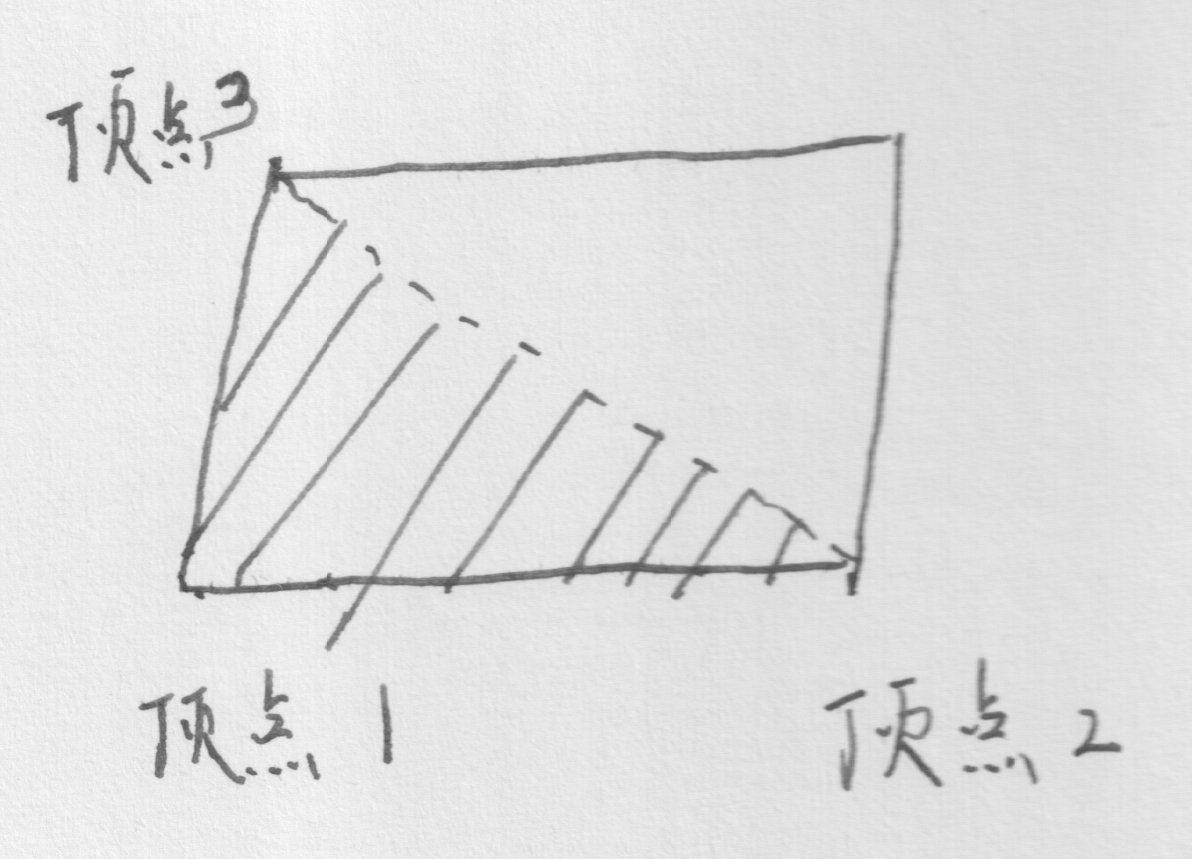
\includegraphics[width=0.4
  \textwidth]{pic1.png} 
  \caption{Surface构造} 
  
\end{figure}

此对象具有以下属性与方法:
\subsection{Surface属性}
\subsubsection{name}
字符串,对象生成时传入,为变量名
\subsubsection{x,y,z}
Sympy变量,创建对象时生成,为坐标
\subsubsection{coords}
列表,元素按顺序为Surface.x,Surface.y,Surface.z
\subsubsection{point,diag0,diag1}
列表,按顺序为顶点1,顶点2,顶点3的坐标
\subsubsection{vec0,vec1}
列表,分别为顶点1指向顶点2,顶点1指向顶点3的向量
\subsubsection{point1}
列表,平行四边形的第四个顶点,由前三个顶点计算得出
\subsubsection{nvec}
列表,平面的法向量,由向量叉乘计算得出,朝向不确定,获取确定朝向的法向量应当使用Surface.rnvec方法
\subsection{Surface方法}
\subsubsection{rnvec(source,wind)}
此方法接受两个变量,按顺序为最近的气体源坐标和Wind对象,返回一个向量(三元列表),为指向气体源头方向的平面法向量,如图所示

\begin{figure}[h] 
  \centering
  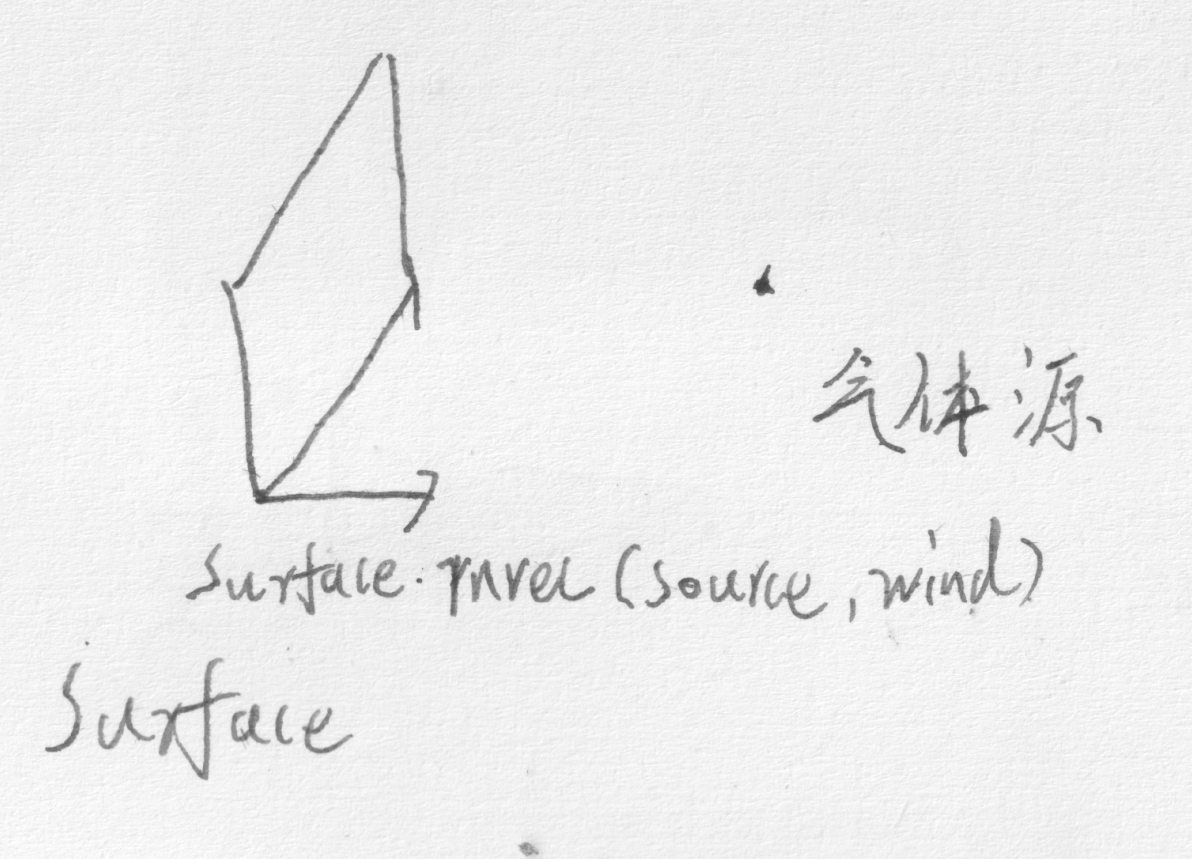
\includegraphics[width=0.55
  \textwidth]{pic2.png} 
  \caption{Surface.rnvec()} 
  
\end{figure}

\section{Cube}
此对象描述各种反射平面造成的反射效果,接受五个变量。按照顺序分别为变量名,一个Surface对象,源点坐标,Wind对象,及一具有默认值3的长度变量,描述反射平面的影响距离,此对象将描述一将Surface描述的面沿朝向法向量的方向平移长度数个单位所扫过的平行六面体,如图所示

\begin{figure}[h] 
  \centering
  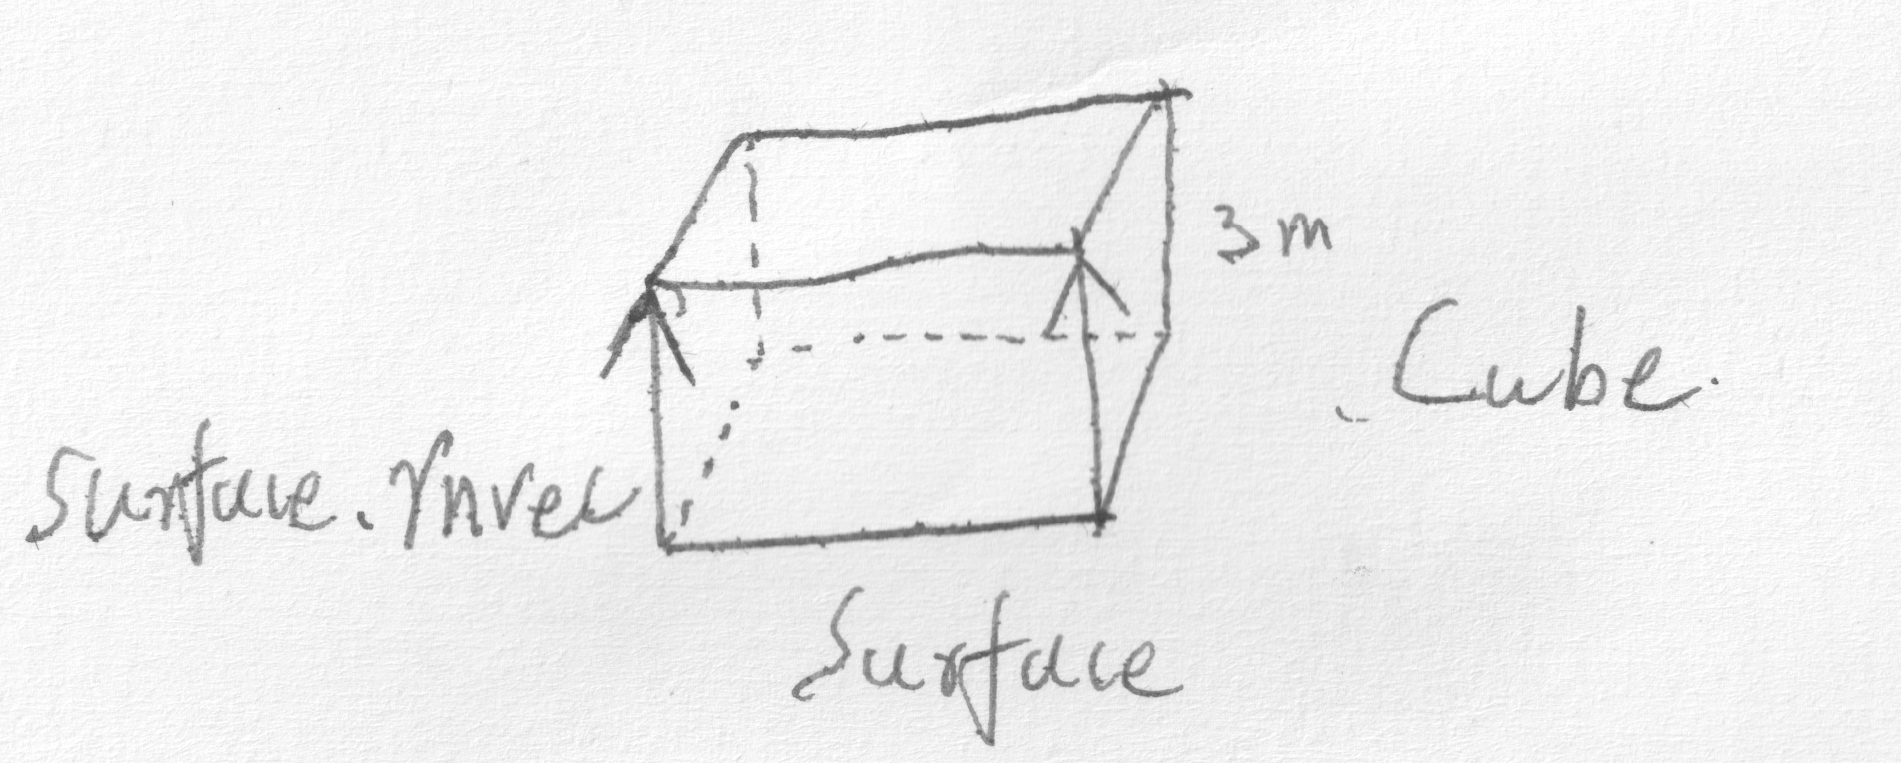
\includegraphics[width=0.8
  \textwidth]{pic3.png} 
  \caption{由Surface生成Cube(长度变量取3)} 
  
\end{figure}

此对象具有如下属性和方法:
\subsection{Cube属性}
\subsubsection{name}
字符串,对象生成时传入,为变量名
\subsubsection{x,y,z}
Sympy变量,创建对象时生成,为坐标
\subsubsection{abscoords}
列表,元素按顺序为Cube.x,Cube.y,Cube.z,为强调此坐标数值为世界坐标系数值而取此名
\subsubsection{surface}
Surface对象
\subsection{Cube方法}
\subsubsection{get\_reflect(leng=3)}
此方法接收一具有默认值3的变量,返回一个Sympy.Piecewise分段函数表达式,其仅在前述的立体空间内具有非0值,具体为一沿法线方向的指数衰减函数。
\subsubsection{get\_decrease(leng=3)}
此方法接收一具有默认值3的变量,返回一个Sympy.Piecewise分段函数表达式,为上一方法返回的函数关于Surface对称的函数。
\section{EnvDiscriptor}
此对象整合所有Cube对象描述的空间,接受两个变量,分别为变量名与一个列表,此列表的组成元素为不定数量个Cube对象。对于一次运行,应当仅存在一个EnvDiscriptor对象

此对象具有如下属性及方法:
\subsection{EnvDiscriptor属性}
\subsubsection{name}
字符串,对象生成时传入,为变量名
\subsubsection{x,y,z}
Sympy变量,创建对象时生成,为坐标
\subsubsection{coords}
列表,元素按顺序为EnvDiscriptor.x,EnvDiscriptor.y,EnvDiscriptor.z
\subsubsection{expr,decrease}
Sympy表达式,分别为Cube.get\_reflect()与Cube.get\_decrease()方法返回的表达式的叠加
\subsection{get\_expr()}
此方法不接受变量,返回EnvDescriptor.expr
\subsection{get\_reflect()}
此方法不接受变量,返回EnvDescriptor.reflect

\section{GaussModel}
生成一个描述具有单位浓度的衰减点源在自由空间内扩散的对象,创建时接受一个变量,为气体源的坐标,此对象具有如下属性及方法
\subsection{GaussModel属性}
\subsubsection{name}
字符串,对象生成时传入,为变量名
\subsubsection{x,y,z}
Sympy变量,创建对象时生成,为坐标
\subsubsection{t}
Sympy变量,创建对象时生成,为时间
\subsubsection{D}
Sympy变量,创建对象时生成,为扩散系数
\subsubsection{expr}
Sympy表达式,描述衰减点源在自由空间内扩散,使用前述Sympy变量构建。
\subsection{GaussModel方法}
\subsubsection{get\_expr()}
此方法不接受变量,返回GaussModel.expr
\subsubsection{coeff\_expr(wind)}
此方法接受一个Wind对象,返回一个Sympy表达式,描述在风与自由扩散共同作用下的浓度变化
\section{Dgas}
此对象为反映不同温度,压强下的扩散系数并进行修正,创建时接受一个变量,为25摄氏度,101千帕时的扩散系数,此对象具有如下属性和方法:
\subsection{Dgas属性}
\subsubsection{name}
字符串,对象生成时传入,为变量名
\subsubsection{std\_val}
数值,为25摄氏度,101千帕时的扩散系数
\subsection{Dgas方法}
\subsubsection{get\_cor\_val(abs\_tmpr=273.15+25,prss=101)}
此方法接受两个具有默认值的变量,均为数值,按顺序为温度与压强,单位分别为摄氏度与千帕,当不带参数调用时返回标准值,带参数调用时返回修正值。
\section{GasMonitor}
此对象反映某一气体传感器的测量结果,创建时接受两个变量,分别为先前记录的数据与传感器的位置,类型均为列表,先前数据要求至少31条。此对象具有以下属性与方法
\subsection{GasMonitor属性}
\subsubsection{data}
列表,其至少需要31条先前数据且最新数据在列表首位
\subsubsection{position}
列表,传感器安装位置的坐标
\subsection{GasMonitor方法}
\subsubsection{test()}
此方法不接受变量,返回一个数值,当为0时表示最新数据在均值的$3\sigma$范围以内,为1时超出均值$3\sigma$,为-1时小于均值$3\sigma$
\subsubsection{get\_newval()}
此方法不接受变量,返回一个数值,为传感器得到的最新数据
\section{Predictor}
此对项为预测用对象,创建时接受一个变量为变量名,此对象具有如下属性及方法:
\subsection{Predictor属性}
\subsubsection{name}
字符串,对象生成时传入,为变量名
\subsubsection{x,y,z}
Sympy变量,创建对象时生成,为坐标
\subsubsection{t}
Sympy变量,创建对象时生成,为时间
\subsection{coords}
列表,其元素按顺序为Predictor.x,Predictor.y,Predictor.z,Predictor.t
\subsection{Predictor方法}
\subsubsection{get\_value(gauss\_model,gas\_monitor,\\env\_discriptor,dgas,temp,pres,wind,coords,time)}
传入九个参数,按顺序分别为GaussModel对象 ,GasMonitor对象EnvDiscriptor对象,Dgas对象,当前温度,当前压强,Wind对象,所要预测的点位的空间坐标列表,所要预测的时间.返回一个数值为符合前述条件的预测浓度值
\end{document}